\section{Background}
\subsection{SIMD}

SIMD stands for Single Instruction Multiple Data.  This is a parallelisation
technique where the program issues a single instruction such as an ADD to the
CPU core, which is then applied to multiple pieces of data at once.  By doing
this any workflow that can be re-written to use the same series of instructions
on a set of data can be sped up a lot.  The most common example of this type of
parallelism is in Graphics Processing Units (GPUs)
\cite{Fatahalian:2008:CLG:1400181.1400197}, these are required to perform the
same transformation to millions of polygons simultaneously and so by utilising
an SIMD architecture consisting of literally hundreds of parallel units they
obtain massive speed ups.

The basic implementation of an SIMD processor is to 

\subsection{Leros}
In order to avoid carrying out redundant work, a decision was made to utilise an
existing solution as a base for development. The advantages were twofold; not only
did it allow for much faster development, but it has already been tested extensively.
 OpenCores\footnote{\url{http://www.opencores.com}}
is a large open-source hardware community, well-known for its collection of hardware solutions for
FPGAs and ASICs in both VHDL and Verilog. Our requirements called for a VHDL
microcontroller, of which there were many to choose from. Other criteria included
simplicity of code, small project size, and a RISC architecture. One project stood out
after applying these critera, named the \emph{Leros} microcontroller after the
Greek Island Leros \cite{schoeberlleros} where the author wrote it.  The Leros MCU is a 16-bit
processor optimized for FPGAs \cite{schoeberlleros} and the design is portable
to the FPGAs of many manufacturers.

Leros is a stable
project and can even be programmed in a restricted subset of Java. It is licenced
under the permissive BSD licence and has been tested under the Xilinx toolchain.
Leros' architecture is a pipelined 16-bit accumulator processor\cite{schoeberlleros},
with instructions executed in a single cycle.

The accumulator architecture made Leros an attractive option for this project due to 
the simplicity a single operand instruction set brings. A second reason that made Leros a strong option was that one of the main goals of Leros was to create a very small simple CPU so that it could be used to investigate different forms of parallel CPU implementation on a reasonably sized FPGA. The small size meant that when implemented on the Spartan Se-1600E it used less then 1\% of the FPGAs resources opening up the possibility of an exceedingly large amount of data to be processed in parallel once the architecture was modified.

A disadvantage of the leros architecture that was not initially realised was that the code had been written with the main emphasis on creating a 16 bit CPU that used as few logic gates as possible. This combined with the fact that all of the coding had been done by a single person meant that the layout of the code left much to be desired. Large amounts of the of the units are implemented inside single processes. An example of this can be found in the code: the ALU, input multiplexer, memory and accumulator are all defined at once in the same process.
 
\begin{figure*}[h]
\center
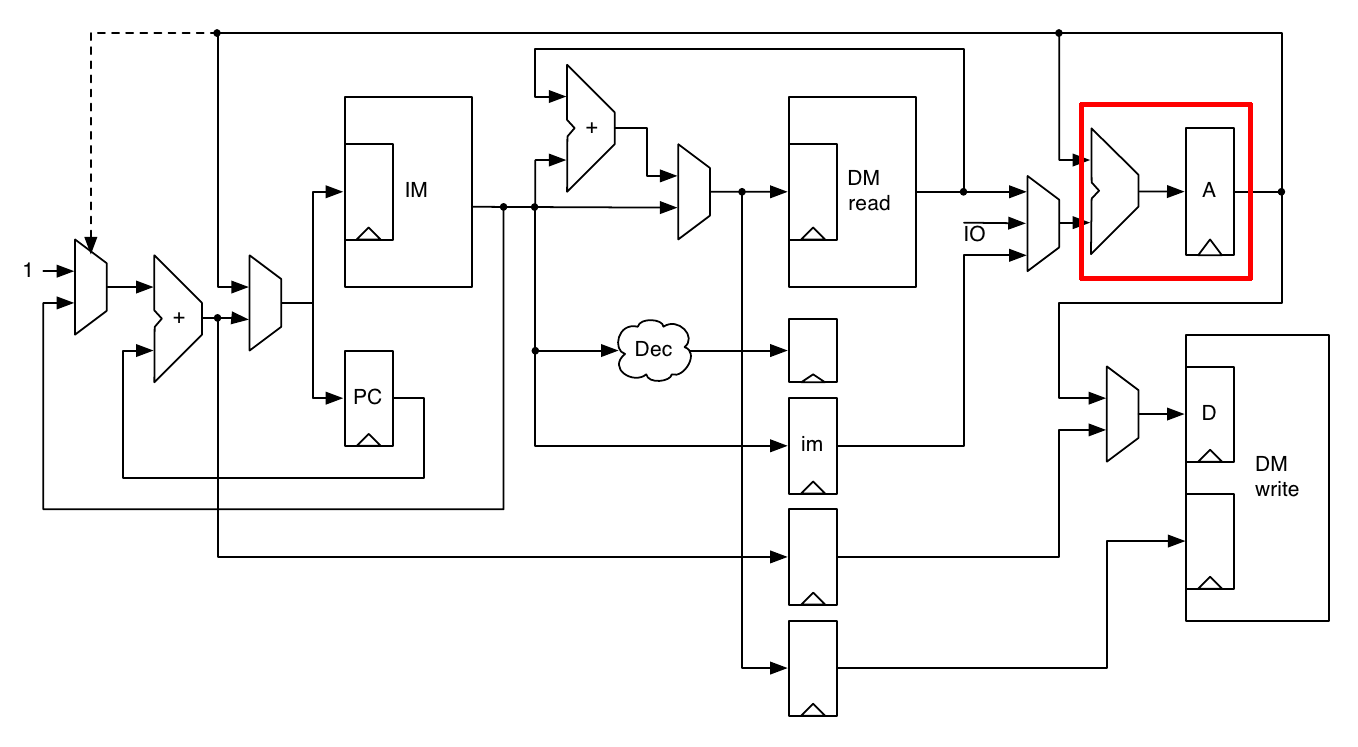
\includegraphics[width=0.9\textwidth]{images/leros-system}
\caption{Leros pipeline. The section of the design to be multiplied has been
highlighted in red. Original image from \cite{schoeberlleros}.
}
\label{fig:leros-system}
\end{figure*}
